\documentclass[11pt,a4paper]{article}
\usepackage[utf8]{inputenc}
\usepackage[T1]{fontenc}
\IfFileExists{spanish.ldf}{\usepackage[spanish,es-nodecimaldot,es-tabla]{babel}}{}
\usepackage{lmodern}
\usepackage[margin=2.5cm]{geometry}
\usepackage{amsmath,amssymb}
\usepackage{graphicx}
\usepackage{booktabs}
\usepackage[output-decimal-marker={,}]{siunitx}
\usepackage{caption}
\usepackage[hidelinks]{hyperref}

\title{Elección de la frecuencia de corte\\del nuevo filtro de temperatura ambiente}
\author{Nicole S. Poliak \\ \small Laboratorio 6/7 --- ITeDA (CNEA-CONICET-UNSAM)}
\date{Noviembre 2026}

\begin{document}
\maketitle

\begin{abstract}
El ítem 5 del plan de trabajo pide construir un filtro no criogénico con una única frecuencia de
corte para todos los canales, que cumpla su función con el menor tiempo de respuesta posible. Se
modela la cadena completa de filtrado con fuente de corriente y se calcula el tiempo que necesita
cada punto de una rampa de corriente. El resultado principal es que, con fuente de corriente, la
velocidad la fija sobre todo la capacidad del filtro y no su frecuencia de corte. Planteando la
elección como un problema de optimización con dos requisitos de atenuación a la frecuencia de
corte del filtro criogénico, se obtiene $R = \SI{330}{\ohm}$ y $C = \SI{330}{\nano\farad}$
($f_c \approx \SI{550}{\hertz}$), que es $2{,}9$ veces más rápido que el filtro usado hasta ahora
para medir corriente de switching.
\end{abstract}

\section{Motivación}

El filtro de temperatura ambiente actual tiene seis configuraciones distintas
(Tabla~5.1 de la tesis de Bazano), con frecuencias de corte entre \SI{180}{\hertz} y
\SI{3962}{\hertz}. El filtro nuevo tiene que tener una sola. Bajar la frecuencia de corte filtra
más, pero hace más lenta la medición: cada punto de una rampa de corriente tiene que esperar a
que la corriente en la juntura se asiente. Para decidir hace falta cuantificar las dos cosas.

La pregunta concreta que motivó el análisis es la siguiente: una rampa de \SI{-1}{\micro\ampere}
a \SI{80}{\micro\ampere} en pasos de \SI{10}{\nano\ampere}, repetida $10^4$ veces (como en la
medición de histogramas de $I_{sw}$), ¿cuánto tarda una medición y cuánto las $10^4$, con cada filtro?

\section{Modelo}

Se usa el modelo ya validado contra LTspice y contra la Tabla~5.1: una escalera R--C en espacio
de estados, plegada al modo diferencial ($R' = 2R_{ta}$, $C' = C_{ta}/2$ en el ambiente;
$R' = 2R_{cry}$, $C' = C_{cry}$ en el criogénico, con $R_{cry} = \SI{22}{\ohm}$ y
$C_{cry} = \SI{47}{\nano\farad}$). La diferencia con el análisis de la tesis es que la excitación
es una \textbf{fuente de corriente} ideal (el Keithley) y la salida es la \textbf{corriente por
la juntura}. Se consideran dos cargas: la juntura en el estado de voltaje cero (un corto; la
inductancia Josephson, $\sim\SI{14}{\pico\henry}$, es despreciable) y en estado normal
($R_N = \SI{74}{\ohm}$), y se toma el peor caso. Con la juntura en voltaje cero el par de
sensado no se carga, así que alcanza con el par de corriente.

\paragraph{Tiempo por punto.} La rampa es una escalera: cada $T$ segundos la corriente sube
$\Delta I$. Por superposición, en régimen el error de la corriente en la juntura al final de cada
punto es
\begin{equation}
  \frac{e(T)}{\Delta I} = \sum_{k=1}^{\infty} r(kT), \qquad
  r(t) = 1 - \frac{y_{\text{escalón}}(t)}{y(\infty)} ,
  \label{eq:escalera}
\end{equation}
donde $r(t)$ es lo que le falta a la respuesta al escalón para llegar a su valor final. Se define
el tiempo por punto como el $T$ que da $e(T) = \varepsilon\,\Delta I$, con $\varepsilon = 1\%$.
Como el sistema es lineal, \textbf{$T$ no depende de $\Delta I$}: si se cambia el paso, solo cambia
la cantidad de puntos. La ecuación~\eqref{eq:escalera} se
verificó contra una simulación temporal de 60 escalones (error $0{,}01006$ contra $0{,}01$).

\section{Tiempos de medición con los filtros actuales}

La Tabla~\ref{tab:fran} responde la pregunta de la motivación. Con pasos de \SI{10}{\nano\ampere}
hay \num{8101} puntos por rampa.

\begin{table}[h]
\centering
\caption{Tiempo por punto ($\varepsilon = 1\%$) y duración de una medición (una rampa de
\SI{-1}{\micro\ampere} a \SI{80}{\micro\ampere} en pasos de \SI{10}{\nano\ampere}) y de $10^4$
mediciones, si cada punto dura lo que pide el filtro. Con \SI{10}{\milli\second} por punto (lo
usado en la tesis) son \SI{81}{\second} y \SI{9.4}{días} para todos los filtros por igual.}
\label{tab:fran}
\begin{tabular}{rrrrrr}
\toprule
$R_{ta}$ [\si{\ohm}] & $C_{ta}$ [\si{\micro\farad}] & $f_c$ [\si{\hertz}] &
$T$ [\si{\milli\second}] & 1 medición & $10^4$ mediciones \\
\midrule
150 & 2,2 &  180 & 3,26 & \SI{26.4}{\second} & 3,1 días \\
150 & 1,0 &  396 & 1,50 & \SI{12.1}{\second} & 1,4 días \\
 51 & 2,2 &  530 & 2,48 & \SI{20.1}{\second} & 2,3 días \\
 51 & 1,0 & 1165 & 1,15 & \SI{9.3}{\second} & 1,1 días \\
 15 & 2,2 & 1801 & 2,23 & \SI{18.1}{\second} & 2,1 días \\
 15 & 1,0 & 3962 & 1,04 & \SI{8.4}{\second} & 23,4 h \\
\midrule
\textbf{330} & \textbf{0,33} & \textbf{547} & \textbf{0,76} & \textbf{\SI{6.1}{\second}} & \textbf{17,0 h} \\
\bottomrule
\end{tabular}
\end{table}

La última fila es el filtro propuesto en la Sección~\ref{sec:eleccion}. En la medición real de
$I_{sw}$ la rampa se corta al saltar y lejos del salto se usan pasos grandes, por lo que los
tiempos absolutos son mucho menores; los cocientes entre filtros no cambian.

Para el filtro de \SI{1801}{\hertz}, que la tesis usó para medir $I_{sw}$ con
\SI{10}{\milli\second} por punto, el modelo pide \SI{2.2}{\milli\second}: ese tiempo estaba
holgado.

\section{La frecuencia de corte no fija la velocidad}

Las frecuencias de corte de la Tabla~\ref{tab:fran} cambian un factor 22, pero los tiempos por
punto solo un factor 3. Con fuente de corriente, la primera $R_{ta}$ no cumple ninguna función (la
fuente empuja la misma corriente igual), y el primer capacitor se descarga a través de todo lo que
hay después: $2R_{ta}$, las tres resistencias criogénicas plegadas ($6R_{cry} = \SI{132}{\ohm}$) y
la juntura. Salvo en los canales de \SI{150}{\ohm}, eso lo dominan el criogénico y la juntura.

La Figura~\ref{fig:tpunto} lo muestra barriendo la $f_c$ a $C$ fija. Cada curva tiene un codo
donde $2R_{ta}$ se hace comparable con $6R_{cry} + R_N \approx \SI{206}{\ohm}$: por encima, subir
la $f_c$ casi no acelera nada; lo que acelera es bajar la $C$.

\begin{figure}[h]
\centering
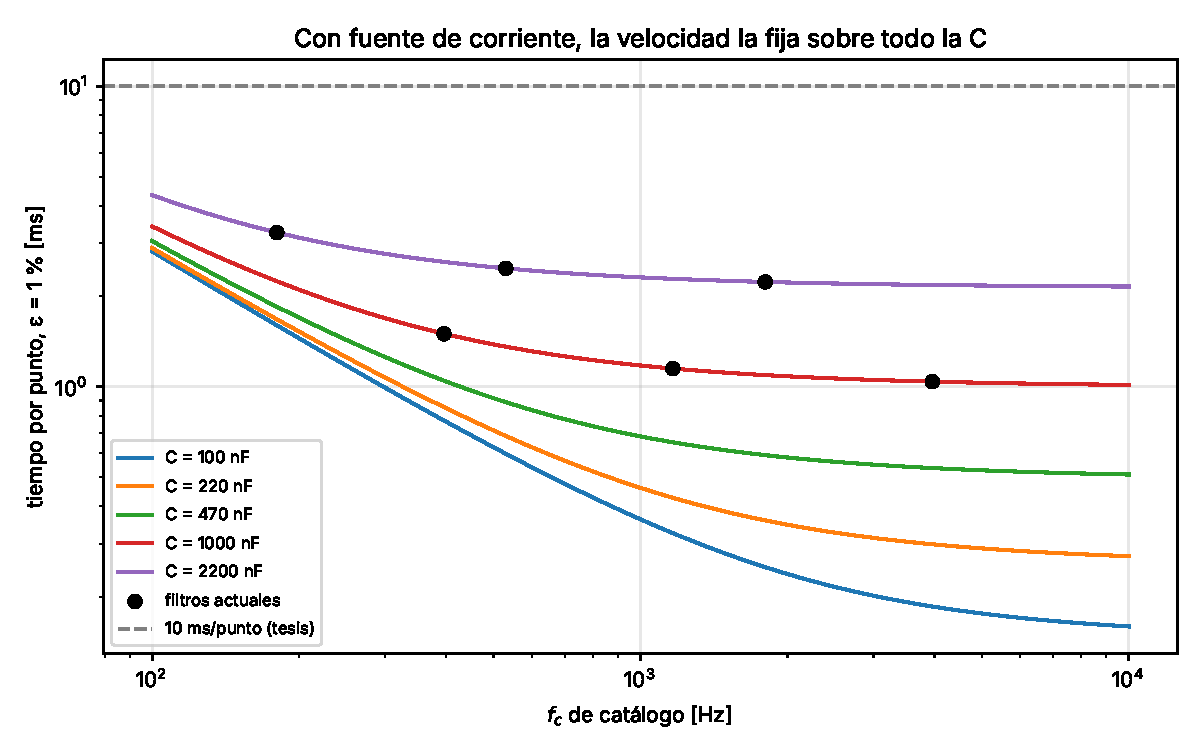
\includegraphics[width=0.85\textwidth]{fig_tpunto_vs_fc.pdf}
\caption{Tiempo por punto en función de la frecuencia de corte de catálogo, para distintas $C$.
Los puntos negros son los seis filtros actuales.}
\label{fig:tpunto}
\end{figure}

\section{Criterio de elección}
\label{sec:eleccion}

Con fuente de corriente, el filtro tiene que frenar dos tipos de ruido y cada uno lo frena una
transferencia distinta:
\begin{itemize}
  \item \textbf{Interferencia de tipo tensión} (pickup en los cables, lazos de masa, lo que viene
  del lado del voltímetro): la frena la transferencia de tensión $H_V$, la de la Tabla~5.1, que
  depende solo de $RC$.
  \item \textbf{Ruido de corriente de la fuente}: lo frena la transferencia de corriente $H_I$, que
  es la misma que fija la velocidad. Un filtro que frena más ruido de corriente es,
  necesariamente, más lento.
\end{itemize}

Se pide una atenuación mínima de las dos a la frecuencia de referencia
$f_{ref} = \SI{28.8}{\kilo\hertz}$, la frecuencia de corte del filtro criogénico: el filtro
ambiente tiene que cubrir la banda en la que el criogénico todavía no actúa. El valor elegido,
\SI{40}{\decibel} para ambas, sale de la medición: con la masa actual, la respuesta medida del
filtro se planta en una meseta de \SIrange{-33}{-47}{\decibel} por encima de
\SI{20}{\kilo\hertz}, de modo que una atenuación mayor no se podría verificar hasta mejorar la
masa.

La elección se plantea como un problema de optimización: entre todas las combinaciones
comerciales ($R$ de la serie E24 entre \SI{10}{\ohm} y \SI{9.1}{\kilo\ohm}, $C$ de la serie E6
entre \SI{47}{\nano\farad} y \SI{2.2}{\micro\farad}), minimizar el tiempo por punto sujeto a
$|H_V(f_{ref})| \le \SI{-40}{\decibel}$ y $|H_I(f_{ref})| \le \SI{-40}{\decibel}$.

\begin{figure}[h]
\centering
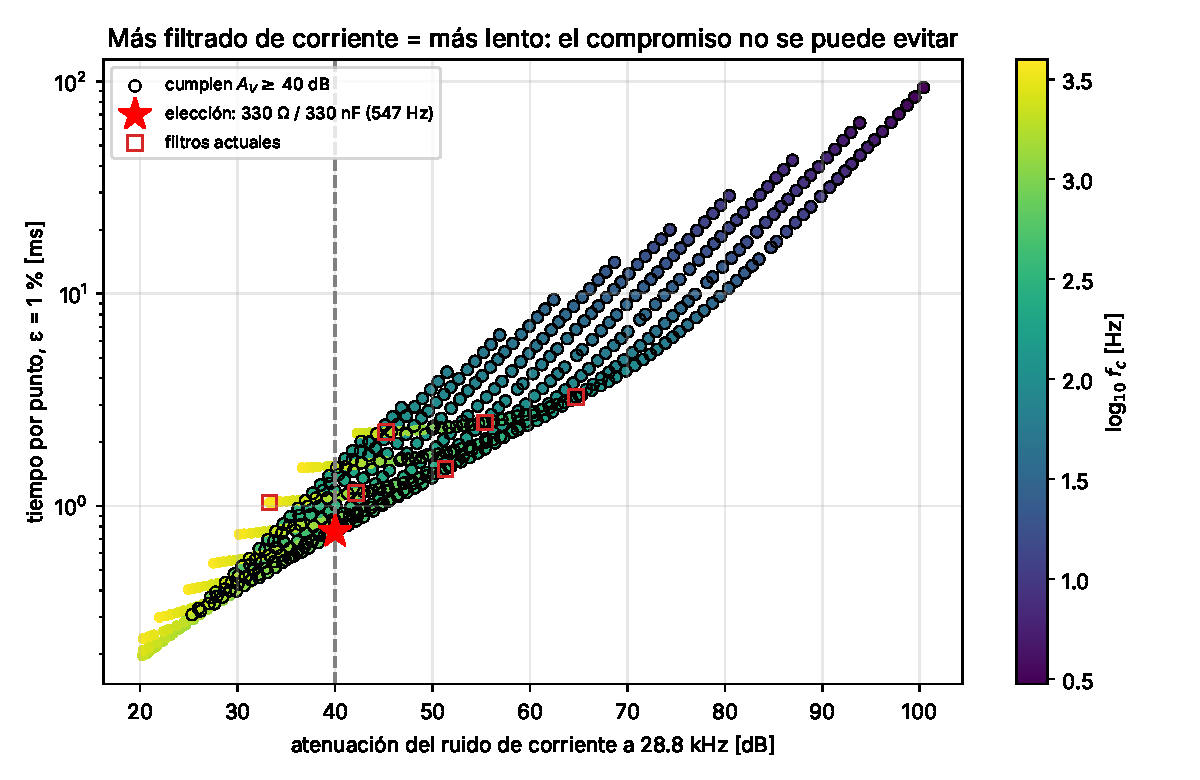
\includegraphics[width=0.85\textwidth]{fig_compromiso.pdf}
\caption{Tiempo por punto contra atenuación del ruido de corriente a \SI{28.8}{\kilo\hertz}, para
las 792 combinaciones comerciales. Los círculos negros cumplen además el requisito de tensión.}
\label{fig:compromiso}
\end{figure}

La Figura~\ref{fig:compromiso} muestra que las combinaciones forman un borde: para cada
atenuación de corriente hay un tiempo mínimo que no se puede bajar. La combinación más rápida que
cumple los dos requisitos es
\begin{equation*}
  R_{ta} = \SI{330}{\ohm}, \qquad C_{ta} = \SI{330}{\nano\farad}, \qquad
  f_c = \SI{547}{\hertz},
\end{equation*}
con $|H_V(f_{ref})| = \SI{-51.9}{\decibel}$, $|H_I(f_{ref})| = \SI{-40.0}{\decibel}$ y
\SI{0.76}{\milli\second} por punto. Frente al filtro de \SI{1801}{\hertz} usado para $I_{sw}$,
es $2{,}9$ veces más rápido, frena \SI{20}{\decibel} más la interferencia de tensión y
\SI{5}{\decibel} menos el ruido de corriente. En la región subgap de la curva IV, donde el tiempo
escala con $R_{sg}C$, el punto pasa de \SI{658}{\milli\second} a \SI{122}{\milli\second}.

El requisito que queda activo es el de corriente: la elección queda justo en
\SI{-40}{\decibel}. Como los capacitores medidos dieron entre un 7 y un 11\,\% por debajo del
nominal, conviene usar capacitores de tolerancia ajustada (film o C0G al 5\,\%).

\subsection*{Sensibilidad}

\begin{table}[h]
\centering
\caption{Elección óptima según los requisitos de atenuación a \SI{28.8}{\kilo\hertz}.}
\label{tab:sens}
\begin{tabular}{rrlrrr}
\toprule
$A_V$ [\si{\decibel}] & $A_I$ [\si{\decibel}] & elección & $f_c$ [\si{\hertz}] &
$T$ [\si{\milli\second}] & 1 medición [\si{\second}] \\
\midrule
30 & 30 & \SI{220}{\ohm} / \SI{220}{\nano\farad} & 1231 & 0,42 & 3,4 \\
40 & 35 & \SI{390}{\ohm} / \SI{220}{\nano\farad} &  694 & 0,57 & 4,6 \\
40 & 40 & \SI{330}{\ohm} / \SI{330}{\nano\farad} &  547 & 0,76 & 6,1 \\
40 & 45 & \SI{160}{\ohm} / \SI{680}{\nano\farad} &  547 & 1,06 & 8,6 \\
50 & 30 & \SI{2.2}{\kilo\ohm} / \SI{47}{\nano\farad} & 576 & 0,52 & 4,2 \\
\bottomrule
\end{tabular}
\end{table}

La Tabla~\ref{tab:sens} muestra que la elección depende sobre todo del requisito de corriente
$A_I$. Con $A_I = \SI{40}{\decibel}$ el resultado no cambia entre $A_V = 30$ y \SI{50}{\decibel}.

\section{Supuestos y pasos siguientes}

\begin{itemize}
  \item No se incluyó la resistencia del cableado del criostato. Con las líneas no
  superconductoras, suma resistencia aguas abajo y hace todo más lento.
  \item No se incluyó el par de sensado, que en estado normal y subgap carga el nodo de la
  juntura y alarga los tiempos.
  \item La fuente de corriente se tomó ideal. El requisito de corriente debería apoyarse en el
  ruido real de la fuente, medido con el analizador de espectro.
  \item Los requisitos de \SI{40}{\decibel} están atados a la masa actual. Si se mejora la
  conexión a masa (ver el análisis del salto del filtro ambiente), se puede pedir más atenuación y
  re-correr la optimización.
\end{itemize}

El cálculo completo está en \texttt{programar/eleccion\_fc\_filtro\_nuevo.ipynb}. Los requisitos
son parámetros al principio del Paso~5, así que la elección se actualiza re-corriendo el notebook.

\end{document}
